
% Default to the notebook output style

    


% Inherit from the specified cell style.




    
\documentclass[11pt]{article}

    
    
    \usepackage[T1]{fontenc}
    % Nicer default font (+ math font) than Computer Modern for most use cases
    \usepackage{mathpazo}

    % Basic figure setup, for now with no caption control since it's done
    % automatically by Pandoc (which extracts ![](path) syntax from Markdown).
    \usepackage{graphicx}
    % We will generate all images so they have a width \maxwidth. This means
    % that they will get their normal width if they fit onto the page, but
    % are scaled down if they would overflow the margins.
    \makeatletter
    \def\maxwidth{\ifdim\Gin@nat@width>\linewidth\linewidth
    \else\Gin@nat@width\fi}
    \makeatother
    \let\Oldincludegraphics\includegraphics
    % Set max figure width to be 80% of text width, for now hardcoded.
    \renewcommand{\includegraphics}[1]{\Oldincludegraphics[width=.8\maxwidth]{#1}}
    % Ensure that by default, figures have no caption (until we provide a
    % proper Figure object with a Caption API and a way to capture that
    % in the conversion process - todo).
    \usepackage{caption}
    \DeclareCaptionLabelFormat{nolabel}{}
    \captionsetup{labelformat=nolabel}

    \usepackage{adjustbox} % Used to constrain images to a maximum size 
    \usepackage{xcolor} % Allow colors to be defined
    \usepackage{enumerate} % Needed for markdown enumerations to work
    \usepackage{geometry} % Used to adjust the document margins
    \usepackage{amsmath} % Equations
    \usepackage{amssymb} % Equations
    \usepackage{textcomp} % defines textquotesingle
    % Hack from http://tex.stackexchange.com/a/47451/13684:
    \AtBeginDocument{%
        \def\PYZsq{\textquotesingle}% Upright quotes in Pygmentized code
    }
    \usepackage{upquote} % Upright quotes for verbatim code
    \usepackage{eurosym} % defines \euro
    \usepackage[mathletters]{ucs} % Extended unicode (utf-8) support
    \usepackage[utf8x]{inputenc} % Allow utf-8 characters in the tex document
    \usepackage{fancyvrb} % verbatim replacement that allows latex
    \usepackage{grffile} % extends the file name processing of package graphics 
                         % to support a larger range 
    % The hyperref package gives us a pdf with properly built
    % internal navigation ('pdf bookmarks' for the table of contents,
    % internal cross-reference links, web links for URLs, etc.)
    \usepackage{hyperref}
    \usepackage{longtable} % longtable support required by pandoc >1.10
    \usepackage{booktabs}  % table support for pandoc > 1.12.2
    \usepackage[inline]{enumitem} % IRkernel/repr support (it uses the enumerate* environment)
    \usepackage[normalem]{ulem} % ulem is needed to support strikethroughs (\sout)
                                % normalem makes italics be italics, not underlines
    

    
    
    % Colors for the hyperref package
    \definecolor{urlcolor}{rgb}{0,.145,.698}
    \definecolor{linkcolor}{rgb}{.71,0.21,0.01}
    \definecolor{citecolor}{rgb}{.12,.54,.11}

    % ANSI colors
    \definecolor{ansi-black}{HTML}{3E424D}
    \definecolor{ansi-black-intense}{HTML}{282C36}
    \definecolor{ansi-red}{HTML}{E75C58}
    \definecolor{ansi-red-intense}{HTML}{B22B31}
    \definecolor{ansi-green}{HTML}{00A250}
    \definecolor{ansi-green-intense}{HTML}{007427}
    \definecolor{ansi-yellow}{HTML}{DDB62B}
    \definecolor{ansi-yellow-intense}{HTML}{B27D12}
    \definecolor{ansi-blue}{HTML}{208FFB}
    \definecolor{ansi-blue-intense}{HTML}{0065CA}
    \definecolor{ansi-magenta}{HTML}{D160C4}
    \definecolor{ansi-magenta-intense}{HTML}{A03196}
    \definecolor{ansi-cyan}{HTML}{60C6C8}
    \definecolor{ansi-cyan-intense}{HTML}{258F8F}
    \definecolor{ansi-white}{HTML}{C5C1B4}
    \definecolor{ansi-white-intense}{HTML}{A1A6B2}

    % commands and environments needed by pandoc snippets
    % extracted from the output of `pandoc -s`
    \providecommand{\tightlist}{%
      \setlength{\itemsep}{0pt}\setlength{\parskip}{0pt}}
    \DefineVerbatimEnvironment{Highlighting}{Verbatim}{commandchars=\\\{\}}
    % Add ',fontsize=\small' for more characters per line
    \newenvironment{Shaded}{}{}
    \newcommand{\KeywordTok}[1]{\textcolor[rgb]{0.00,0.44,0.13}{\textbf{{#1}}}}
    \newcommand{\DataTypeTok}[1]{\textcolor[rgb]{0.56,0.13,0.00}{{#1}}}
    \newcommand{\DecValTok}[1]{\textcolor[rgb]{0.25,0.63,0.44}{{#1}}}
    \newcommand{\BaseNTok}[1]{\textcolor[rgb]{0.25,0.63,0.44}{{#1}}}
    \newcommand{\FloatTok}[1]{\textcolor[rgb]{0.25,0.63,0.44}{{#1}}}
    \newcommand{\CharTok}[1]{\textcolor[rgb]{0.25,0.44,0.63}{{#1}}}
    \newcommand{\StringTok}[1]{\textcolor[rgb]{0.25,0.44,0.63}{{#1}}}
    \newcommand{\CommentTok}[1]{\textcolor[rgb]{0.38,0.63,0.69}{\textit{{#1}}}}
    \newcommand{\OtherTok}[1]{\textcolor[rgb]{0.00,0.44,0.13}{{#1}}}
    \newcommand{\AlertTok}[1]{\textcolor[rgb]{1.00,0.00,0.00}{\textbf{{#1}}}}
    \newcommand{\FunctionTok}[1]{\textcolor[rgb]{0.02,0.16,0.49}{{#1}}}
    \newcommand{\RegionMarkerTok}[1]{{#1}}
    \newcommand{\ErrorTok}[1]{\textcolor[rgb]{1.00,0.00,0.00}{\textbf{{#1}}}}
    \newcommand{\NormalTok}[1]{{#1}}
    
    % Additional commands for more recent versions of Pandoc
    \newcommand{\ConstantTok}[1]{\textcolor[rgb]{0.53,0.00,0.00}{{#1}}}
    \newcommand{\SpecialCharTok}[1]{\textcolor[rgb]{0.25,0.44,0.63}{{#1}}}
    \newcommand{\VerbatimStringTok}[1]{\textcolor[rgb]{0.25,0.44,0.63}{{#1}}}
    \newcommand{\SpecialStringTok}[1]{\textcolor[rgb]{0.73,0.40,0.53}{{#1}}}
    \newcommand{\ImportTok}[1]{{#1}}
    \newcommand{\DocumentationTok}[1]{\textcolor[rgb]{0.73,0.13,0.13}{\textit{{#1}}}}
    \newcommand{\AnnotationTok}[1]{\textcolor[rgb]{0.38,0.63,0.69}{\textbf{\textit{{#1}}}}}
    \newcommand{\CommentVarTok}[1]{\textcolor[rgb]{0.38,0.63,0.69}{\textbf{\textit{{#1}}}}}
    \newcommand{\VariableTok}[1]{\textcolor[rgb]{0.10,0.09,0.49}{{#1}}}
    \newcommand{\ControlFlowTok}[1]{\textcolor[rgb]{0.00,0.44,0.13}{\textbf{{#1}}}}
    \newcommand{\OperatorTok}[1]{\textcolor[rgb]{0.40,0.40,0.40}{{#1}}}
    \newcommand{\BuiltInTok}[1]{{#1}}
    \newcommand{\ExtensionTok}[1]{{#1}}
    \newcommand{\PreprocessorTok}[1]{\textcolor[rgb]{0.74,0.48,0.00}{{#1}}}
    \newcommand{\AttributeTok}[1]{\textcolor[rgb]{0.49,0.56,0.16}{{#1}}}
    \newcommand{\InformationTok}[1]{\textcolor[rgb]{0.38,0.63,0.69}{\textbf{\textit{{#1}}}}}
    \newcommand{\WarningTok}[1]{\textcolor[rgb]{0.38,0.63,0.69}{\textbf{\textit{{#1}}}}}
    
    
    % Define a nice break command that doesn't care if a line doesn't already
    % exist.
    \def\br{\hspace*{\fill} \\* }
    % Math Jax compatability definitions
    \def\gt{>}
    \def\lt{<}
    % Document parameters
    \title{Quantum Edge Detection Demo}
    \author{Paul Kassebaum}
   
    
    

    % Pygments definitions
    
\makeatletter
\def\PY@reset{\let\PY@it=\relax \let\PY@bf=\relax%
    \let\PY@ul=\relax \let\PY@tc=\relax%
    \let\PY@bc=\relax \let\PY@ff=\relax}
\def\PY@tok#1{\csname PY@tok@#1\endcsname}
\def\PY@toks#1+{\ifx\relax#1\empty\else%
    \PY@tok{#1}\expandafter\PY@toks\fi}
\def\PY@do#1{\PY@bc{\PY@tc{\PY@ul{%
    \PY@it{\PY@bf{\PY@ff{#1}}}}}}}
\def\PY#1#2{\PY@reset\PY@toks#1+\relax+\PY@do{#2}}

\expandafter\def\csname PY@tok@w\endcsname{\def\PY@tc##1{\textcolor[rgb]{0.73,0.73,0.73}{##1}}}
\expandafter\def\csname PY@tok@c\endcsname{\let\PY@it=\textit\def\PY@tc##1{\textcolor[rgb]{0.25,0.50,0.50}{##1}}}
\expandafter\def\csname PY@tok@cp\endcsname{\def\PY@tc##1{\textcolor[rgb]{0.74,0.48,0.00}{##1}}}
\expandafter\def\csname PY@tok@k\endcsname{\let\PY@bf=\textbf\def\PY@tc##1{\textcolor[rgb]{0.00,0.50,0.00}{##1}}}
\expandafter\def\csname PY@tok@kp\endcsname{\def\PY@tc##1{\textcolor[rgb]{0.00,0.50,0.00}{##1}}}
\expandafter\def\csname PY@tok@kt\endcsname{\def\PY@tc##1{\textcolor[rgb]{0.69,0.00,0.25}{##1}}}
\expandafter\def\csname PY@tok@o\endcsname{\def\PY@tc##1{\textcolor[rgb]{0.40,0.40,0.40}{##1}}}
\expandafter\def\csname PY@tok@ow\endcsname{\let\PY@bf=\textbf\def\PY@tc##1{\textcolor[rgb]{0.67,0.13,1.00}{##1}}}
\expandafter\def\csname PY@tok@nb\endcsname{\def\PY@tc##1{\textcolor[rgb]{0.00,0.50,0.00}{##1}}}
\expandafter\def\csname PY@tok@nf\endcsname{\def\PY@tc##1{\textcolor[rgb]{0.00,0.00,1.00}{##1}}}
\expandafter\def\csname PY@tok@nc\endcsname{\let\PY@bf=\textbf\def\PY@tc##1{\textcolor[rgb]{0.00,0.00,1.00}{##1}}}
\expandafter\def\csname PY@tok@nn\endcsname{\let\PY@bf=\textbf\def\PY@tc##1{\textcolor[rgb]{0.00,0.00,1.00}{##1}}}
\expandafter\def\csname PY@tok@ne\endcsname{\let\PY@bf=\textbf\def\PY@tc##1{\textcolor[rgb]{0.82,0.25,0.23}{##1}}}
\expandafter\def\csname PY@tok@nv\endcsname{\def\PY@tc##1{\textcolor[rgb]{0.10,0.09,0.49}{##1}}}
\expandafter\def\csname PY@tok@no\endcsname{\def\PY@tc##1{\textcolor[rgb]{0.53,0.00,0.00}{##1}}}
\expandafter\def\csname PY@tok@nl\endcsname{\def\PY@tc##1{\textcolor[rgb]{0.63,0.63,0.00}{##1}}}
\expandafter\def\csname PY@tok@ni\endcsname{\let\PY@bf=\textbf\def\PY@tc##1{\textcolor[rgb]{0.60,0.60,0.60}{##1}}}
\expandafter\def\csname PY@tok@na\endcsname{\def\PY@tc##1{\textcolor[rgb]{0.49,0.56,0.16}{##1}}}
\expandafter\def\csname PY@tok@nt\endcsname{\let\PY@bf=\textbf\def\PY@tc##1{\textcolor[rgb]{0.00,0.50,0.00}{##1}}}
\expandafter\def\csname PY@tok@nd\endcsname{\def\PY@tc##1{\textcolor[rgb]{0.67,0.13,1.00}{##1}}}
\expandafter\def\csname PY@tok@s\endcsname{\def\PY@tc##1{\textcolor[rgb]{0.73,0.13,0.13}{##1}}}
\expandafter\def\csname PY@tok@sd\endcsname{\let\PY@it=\textit\def\PY@tc##1{\textcolor[rgb]{0.73,0.13,0.13}{##1}}}
\expandafter\def\csname PY@tok@si\endcsname{\let\PY@bf=\textbf\def\PY@tc##1{\textcolor[rgb]{0.73,0.40,0.53}{##1}}}
\expandafter\def\csname PY@tok@se\endcsname{\let\PY@bf=\textbf\def\PY@tc##1{\textcolor[rgb]{0.73,0.40,0.13}{##1}}}
\expandafter\def\csname PY@tok@sr\endcsname{\def\PY@tc##1{\textcolor[rgb]{0.73,0.40,0.53}{##1}}}
\expandafter\def\csname PY@tok@ss\endcsname{\def\PY@tc##1{\textcolor[rgb]{0.10,0.09,0.49}{##1}}}
\expandafter\def\csname PY@tok@sx\endcsname{\def\PY@tc##1{\textcolor[rgb]{0.00,0.50,0.00}{##1}}}
\expandafter\def\csname PY@tok@m\endcsname{\def\PY@tc##1{\textcolor[rgb]{0.40,0.40,0.40}{##1}}}
\expandafter\def\csname PY@tok@gh\endcsname{\let\PY@bf=\textbf\def\PY@tc##1{\textcolor[rgb]{0.00,0.00,0.50}{##1}}}
\expandafter\def\csname PY@tok@gu\endcsname{\let\PY@bf=\textbf\def\PY@tc##1{\textcolor[rgb]{0.50,0.00,0.50}{##1}}}
\expandafter\def\csname PY@tok@gd\endcsname{\def\PY@tc##1{\textcolor[rgb]{0.63,0.00,0.00}{##1}}}
\expandafter\def\csname PY@tok@gi\endcsname{\def\PY@tc##1{\textcolor[rgb]{0.00,0.63,0.00}{##1}}}
\expandafter\def\csname PY@tok@gr\endcsname{\def\PY@tc##1{\textcolor[rgb]{1.00,0.00,0.00}{##1}}}
\expandafter\def\csname PY@tok@ge\endcsname{\let\PY@it=\textit}
\expandafter\def\csname PY@tok@gs\endcsname{\let\PY@bf=\textbf}
\expandafter\def\csname PY@tok@gp\endcsname{\let\PY@bf=\textbf\def\PY@tc##1{\textcolor[rgb]{0.00,0.00,0.50}{##1}}}
\expandafter\def\csname PY@tok@go\endcsname{\def\PY@tc##1{\textcolor[rgb]{0.53,0.53,0.53}{##1}}}
\expandafter\def\csname PY@tok@gt\endcsname{\def\PY@tc##1{\textcolor[rgb]{0.00,0.27,0.87}{##1}}}
\expandafter\def\csname PY@tok@err\endcsname{\def\PY@bc##1{\setlength{\fboxsep}{0pt}\fcolorbox[rgb]{1.00,0.00,0.00}{1,1,1}{\strut ##1}}}
\expandafter\def\csname PY@tok@kc\endcsname{\let\PY@bf=\textbf\def\PY@tc##1{\textcolor[rgb]{0.00,0.50,0.00}{##1}}}
\expandafter\def\csname PY@tok@kd\endcsname{\let\PY@bf=\textbf\def\PY@tc##1{\textcolor[rgb]{0.00,0.50,0.00}{##1}}}
\expandafter\def\csname PY@tok@kn\endcsname{\let\PY@bf=\textbf\def\PY@tc##1{\textcolor[rgb]{0.00,0.50,0.00}{##1}}}
\expandafter\def\csname PY@tok@kr\endcsname{\let\PY@bf=\textbf\def\PY@tc##1{\textcolor[rgb]{0.00,0.50,0.00}{##1}}}
\expandafter\def\csname PY@tok@bp\endcsname{\def\PY@tc##1{\textcolor[rgb]{0.00,0.50,0.00}{##1}}}
\expandafter\def\csname PY@tok@fm\endcsname{\def\PY@tc##1{\textcolor[rgb]{0.00,0.00,1.00}{##1}}}
\expandafter\def\csname PY@tok@vc\endcsname{\def\PY@tc##1{\textcolor[rgb]{0.10,0.09,0.49}{##1}}}
\expandafter\def\csname PY@tok@vg\endcsname{\def\PY@tc##1{\textcolor[rgb]{0.10,0.09,0.49}{##1}}}
\expandafter\def\csname PY@tok@vi\endcsname{\def\PY@tc##1{\textcolor[rgb]{0.10,0.09,0.49}{##1}}}
\expandafter\def\csname PY@tok@vm\endcsname{\def\PY@tc##1{\textcolor[rgb]{0.10,0.09,0.49}{##1}}}
\expandafter\def\csname PY@tok@sa\endcsname{\def\PY@tc##1{\textcolor[rgb]{0.73,0.13,0.13}{##1}}}
\expandafter\def\csname PY@tok@sb\endcsname{\def\PY@tc##1{\textcolor[rgb]{0.73,0.13,0.13}{##1}}}
\expandafter\def\csname PY@tok@sc\endcsname{\def\PY@tc##1{\textcolor[rgb]{0.73,0.13,0.13}{##1}}}
\expandafter\def\csname PY@tok@dl\endcsname{\def\PY@tc##1{\textcolor[rgb]{0.73,0.13,0.13}{##1}}}
\expandafter\def\csname PY@tok@s2\endcsname{\def\PY@tc##1{\textcolor[rgb]{0.73,0.13,0.13}{##1}}}
\expandafter\def\csname PY@tok@sh\endcsname{\def\PY@tc##1{\textcolor[rgb]{0.73,0.13,0.13}{##1}}}
\expandafter\def\csname PY@tok@s1\endcsname{\def\PY@tc##1{\textcolor[rgb]{0.73,0.13,0.13}{##1}}}
\expandafter\def\csname PY@tok@mb\endcsname{\def\PY@tc##1{\textcolor[rgb]{0.40,0.40,0.40}{##1}}}
\expandafter\def\csname PY@tok@mf\endcsname{\def\PY@tc##1{\textcolor[rgb]{0.40,0.40,0.40}{##1}}}
\expandafter\def\csname PY@tok@mh\endcsname{\def\PY@tc##1{\textcolor[rgb]{0.40,0.40,0.40}{##1}}}
\expandafter\def\csname PY@tok@mi\endcsname{\def\PY@tc##1{\textcolor[rgb]{0.40,0.40,0.40}{##1}}}
\expandafter\def\csname PY@tok@il\endcsname{\def\PY@tc##1{\textcolor[rgb]{0.40,0.40,0.40}{##1}}}
\expandafter\def\csname PY@tok@mo\endcsname{\def\PY@tc##1{\textcolor[rgb]{0.40,0.40,0.40}{##1}}}
\expandafter\def\csname PY@tok@ch\endcsname{\let\PY@it=\textit\def\PY@tc##1{\textcolor[rgb]{0.25,0.50,0.50}{##1}}}
\expandafter\def\csname PY@tok@cm\endcsname{\let\PY@it=\textit\def\PY@tc##1{\textcolor[rgb]{0.25,0.50,0.50}{##1}}}
\expandafter\def\csname PY@tok@cpf\endcsname{\let\PY@it=\textit\def\PY@tc##1{\textcolor[rgb]{0.25,0.50,0.50}{##1}}}
\expandafter\def\csname PY@tok@c1\endcsname{\let\PY@it=\textit\def\PY@tc##1{\textcolor[rgb]{0.25,0.50,0.50}{##1}}}
\expandafter\def\csname PY@tok@cs\endcsname{\let\PY@it=\textit\def\PY@tc##1{\textcolor[rgb]{0.25,0.50,0.50}{##1}}}

\def\PYZbs{\char`\\}
\def\PYZus{\char`\_}
\def\PYZob{\char`\{}
\def\PYZcb{\char`\}}
\def\PYZca{\char`\^}
\def\PYZam{\char`\&}
\def\PYZlt{\char`\<}
\def\PYZgt{\char`\>}
\def\PYZsh{\char`\#}
\def\PYZpc{\char`\%}
\def\PYZdl{\char`\$}
\def\PYZhy{\char`\-}
\def\PYZsq{\char`\'}
\def\PYZdq{\char`\"}
\def\PYZti{\char`\~}
% for compatibility with earlier versions
\def\PYZat{@}
\def\PYZlb{[}
\def\PYZrb{]}
\makeatother


    % Exact colors from NB
    \definecolor{incolor}{rgb}{0.0, 0.0, 0.5}
    \definecolor{outcolor}{rgb}{0.545, 0.0, 0.0}



    
    % Prevent overflowing lines due to hard-to-break entities
    \sloppy 
    % Setup hyperref package
    \hypersetup{
      breaklinks=true,  % so long urls are correctly broken across lines
      colorlinks=true,
      urlcolor=urlcolor,
      linkcolor=linkcolor,
      citecolor=citecolor,
      }
    % Slightly bigger margins than the latex defaults
    
    \geometry{verbose,tmargin=1in,bmargin=1in,lmargin=1in,rmargin=1in}
    
    

    \begin{document}
    
    
    \maketitle
    


    \hypertarget{quantum-edge-detection}{%
\section{Introduction}\label{quantum-edge-detection}}

This demonstration shows how to use \href{https://qiskit.org/}{Qiskit™}
to perform edge detection in images with the quantum Hadamard edge
detection algorithm, which completes the task with just one single-qubit
operation, independent of the size of the image, illustrating the
potential of quantum image processing for highly efficient image and
video processing.

\begin{figure}[h]
\centering
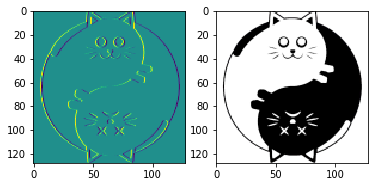
\includegraphics{../img/edge.png}
\end{figure}

    \hypertarget{what-indicates-an-edge}{%
\section{What indicates an edge?}\label{what-indicates-an-edge}}

    Consider the following row of pixels called \(\alpha\):

\[\alpha = [0, 0, 0, 1, 1, 1, 0, 0, 0],\]

\begin{figure}[h]
\centering

\includegraphics{../img/p.png}
\end{figure}

and the difference of its nearest neighboring pixels called
\(\Delta \alpha\)

\[\Delta \alpha = [\alpha_1-\alpha_0, \alpha_2-\alpha_1, \ldots, \alpha_n-\alpha_{n-1},\alpha_0-\alpha_n]\]

\[\Delta \alpha = [0,0,1,0,0,-1,0,0,0]\]

\begin{figure}[h]
\centering

\includegraphics{../img/dp.png}
\end{figure}

The differences \(\Delta \alpha\) take on non-zero values where there
are changes (edges) in the original image \(\alpha\).

So, \(\Delta \alpha\) indicates edges in \(\alpha\).

    \hypertarget{the-hadamard-quantum-gate}{%
\section{The Hadamard Quantum Gate}\label{the-hadamard-quantum-gate}}

    The Hadamard gate has the following effect on the zero and one basis
states of a qubit:

\(H|0\rangle \rightarrow (|0\rangle + |1\rangle)/\sqrt{2}\)

\(H|1\rangle \rightarrow (|0\rangle - |1\rangle)/\sqrt{2}\)

Consider a two pixel image that we represent with a single qubit:

\[|\textrm{image}\rangle = \alpha_0 |0\rangle + \alpha_1 |1\rangle\]

where \(\alpha_0\) is proportional to the value of pixel 0, \(\alpha_1\)
is proportional to the value of pixel 1. The \(\alpha\)'s now also tell
us the probabilty of finding the qubit in state \(|0\rangle\) or
\(|1\rangle\) when we measure it. We will find the qubit in state
\(|0\rangle\) with a probabilty of \(\alpha_0^2\), or in the state
\(|1\rangle\) with probability \(\alpha_1^2\).

    When we apply the Hadamard quantum gate to the image state, it gets
transformed into a new state as follows:

\[H|\textrm{image}\rangle = H \alpha_0 |0\rangle + H \alpha_1 |1\rangle\]

\[H|\textrm{image}\rangle = \alpha_0 H |0\rangle + \alpha_1 H |1\rangle\]

\[H|\textrm{image}\rangle = \alpha_0 (|0\rangle + |1\rangle)/\sqrt{2} + \alpha_1 (|0\rangle - |1\rangle)/\sqrt{2}\]

\[H|\textrm{image}\rangle =  \frac{1}{\sqrt{2}}\left[(\alpha_0 + \alpha_1)|0\rangle + (\alpha_0 - \alpha_1)|1\rangle)\right]\]

Now if we measure the qubit, the probabilty of finding it in state
\(|0\rangle\) is \(P(0) = (\alpha_0 + \alpha_1)^2/2\) and the
probability of finding it in state \(|1\rangle\) is
\(P(1) = (\alpha_0 - \alpha_1)^2/2\).

If the two pixels have the same value, then \(\alpha_0 - \alpha_1 = 0\),
so \(P(1) = 0\). If the two pixels have different values, then
\(P(1) > 0\).

This is a clue that the Hadamard quantum gate can be used to indicate
edges in an image.

    \hypertarget{representing-an-image-as-a-state-vector}{%
\section{Representing an image as a state
vector}\label{representing-an-image-as-a-state-vector}}

    Represent the image as a quantum state as follows

\begin{figure}[h]
\centering
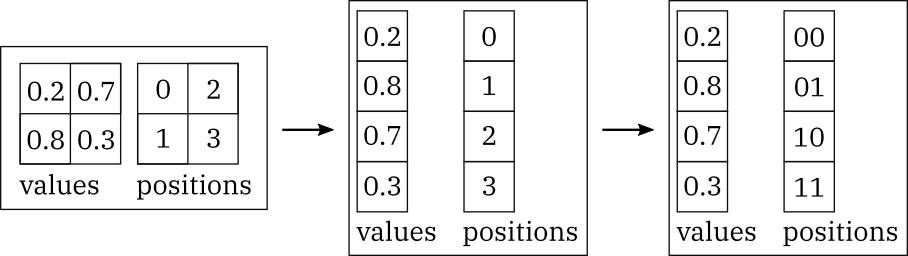
\includegraphics{../img/quantum_encoding.png}
\end{figure}

    The image begins as a matrix of values at certain pixel positions.
Unravel the matrices to form vectors. Then rewrite the pixel positions
from decimal to binary.

The image can then be represented as the quantum state of a two qubit
system:

\[|\textrm{image}\rangle = \frac{0.2 |00\rangle + 0.8 |01\rangle + 0.7 |10\rangle + 0.3 |11\rangle}{\sqrt{0.2^2 + 0.8^2 + 0.7^2 + 0.3^2}}\]

    \hypertarget{programming-the-encoding}{%
\section{Programming the encoding}\label{programming-the-encoding}}

Read the example image in and display it. Get the first color channel of
the image and \texttt{ravel} it to form a column vector.

    \begin{Verbatim}[commandchars=\\\{\}]
{\color{incolor}In [{\color{incolor}1}]:} \PY{k+kn}{import} \PY{n+nn}{numpy} \PY{k}{as} \PY{n+nn}{np}
        \PY{k+kn}{from} \PY{n+nn}{numpy} \PY{k}{import} \PY{n}{pi}
        \PY{k+kn}{import} \PY{n+nn}{matplotlib}\PY{n+nn}{.}\PY{n+nn}{pyplot} \PY{k}{as} \PY{n+nn}{plt}
        \PY{k+kn}{import} \PY{n+nn}{matplotlib}\PY{n+nn}{.}\PY{n+nn}{image}  \PY{k}{as} \PY{n+nn}{mpimg}
        \PY{k+kn}{from} \PY{n+nn}{skimage}\PY{n+nn}{.}\PY{n+nn}{transform} \PY{k}{import} \PY{n}{resize}
\end{Verbatim}


    \begin{Verbatim}[commandchars=\\\{\}]
{\color{incolor}In [{\color{incolor}2}]:} \PY{n}{filename} \PY{o}{=} \PY{l+s+s1}{\PYZsq{}}\PY{l+s+s1}{../img/schrodin\PYZus{}yang.png}\PY{l+s+s1}{\PYZsq{}}
        \PY{n}{im} \PY{o}{=} \PY{n}{mpimg}\PY{o}{.}\PY{n}{imread}\PY{p}{(}\PY{n}{filename}\PY{p}{)}
        
        \PY{n}{n\PYZus{}pixels} \PY{o}{=} \PY{l+m+mi}{2}\PY{o}{*}\PY{o}{*}\PY{l+m+mi}{5}
        \PY{n}{im} \PY{o}{=} \PY{n}{resize}\PY{p}{(}\PY{n}{im}\PY{p}{,} \PY{p}{(}\PY{n}{n\PYZus{}pixels}\PY{p}{,} \PY{n}{n\PYZus{}pixels}\PY{p}{)}\PY{p}{)}
        
        \PY{n}{data} \PY{o}{=} \PY{n}{im}\PY{p}{[}\PY{p}{:}\PY{p}{,}\PY{p}{:}\PY{p}{,}\PY{l+m+mi}{0}\PY{p}{]}\PY{o}{.}\PY{n}{ravel}\PY{p}{(}\PY{p}{)}
        
        \PY{n}{fig}\PY{p}{,} \PY{n}{ax} \PY{o}{=} \PY{n}{plt}\PY{o}{.}\PY{n}{subplots}\PY{p}{(}\PY{p}{)}
        \PY{n}{ax}\PY{o}{.}\PY{n}{imshow}\PY{p}{(}\PY{n}{im}\PY{p}{)}
\end{Verbatim}


\begin{Verbatim}[commandchars=\\\{\}]
{\color{outcolor}Out[{\color{outcolor}2}]:} <matplotlib.image.AxesImage at 0x1c21decdd8>
\end{Verbatim}
            
    \begin{center}
    \adjustimage{max size={0.9\linewidth}{0.9\paperheight}}{../img/output_12_1.png}
    \end{center}
    { \hspace*{\fill} \\}
    
    Use Qiskit Aqua to encode the image as a quantum state.

    \begin{Verbatim}[commandchars=\\\{\}]
{\color{incolor}In [{\color{incolor}4}]:} \PY{n}{n\PYZus{}qubits} \PY{o}{=} \PY{n+nb}{int}\PY{p}{(}\PY{n}{np}\PY{o}{.}\PY{n}{log2}\PY{p}{(}\PY{n+nb}{len}\PY{p}{(}\PY{n}{data}\PY{p}{)}\PY{p}{)}\PY{p}{)}
        
        \PY{k+kn}{from} \PY{n+nn}{qiskit\PYZus{}aqua}\PY{n+nn}{.}\PY{n+nn}{components}\PY{n+nn}{.}\PY{n+nn}{initial\PYZus{}states} \PY{k}{import} \PY{n}{Custom}
        \PY{n}{init\PYZus{}state} \PY{o}{=} \PY{n}{Custom}\PY{p}{(}\PY{n}{n\PYZus{}qubits}\PY{p}{,} \PY{n}{state\PYZus{}vector}\PY{o}{=}\PY{n}{data}\PY{p}{)}
\end{Verbatim}


    Get the quantum circuit \texttt{circ} that creates the image
representation and its quantum register \texttt{qr} containing qubits.
The circuit's register begins in the zero state
\(|000\ldots 000\rangle\) (as many zeros as there are qubits) that get
modified by quantum gates to end up in the state that represents the
image, \(|\textrm{image}\rangle\).

    \begin{Verbatim}[commandchars=\\\{\}]
{\color{incolor}In [{\color{incolor}5}]:} \PY{n}{circ} \PY{o}{=} \PY{n}{init\PYZus{}state}\PY{o}{.}\PY{n}{construct\PYZus{}circuit}\PY{p}{(}\PY{l+s+s1}{\PYZsq{}}\PY{l+s+s1}{circuit}\PY{l+s+s1}{\PYZsq{}}\PY{p}{)}
        \PY{n}{qr}   \PY{o}{=} \PY{n}{circ}\PY{o}{.}\PY{n}{qregs}
\end{Verbatim}


    The series of quantum gates (the quantum circuit) for a 4x4 version of
the image is

    \begin{Verbatim}[commandchars=\\\{\}]
{\color{incolor}In [{\color{incolor}6}]:} \PY{c+c1}{\PYZsh{} circ.draw()}
\end{Verbatim}


    \begin{figure}
\centering
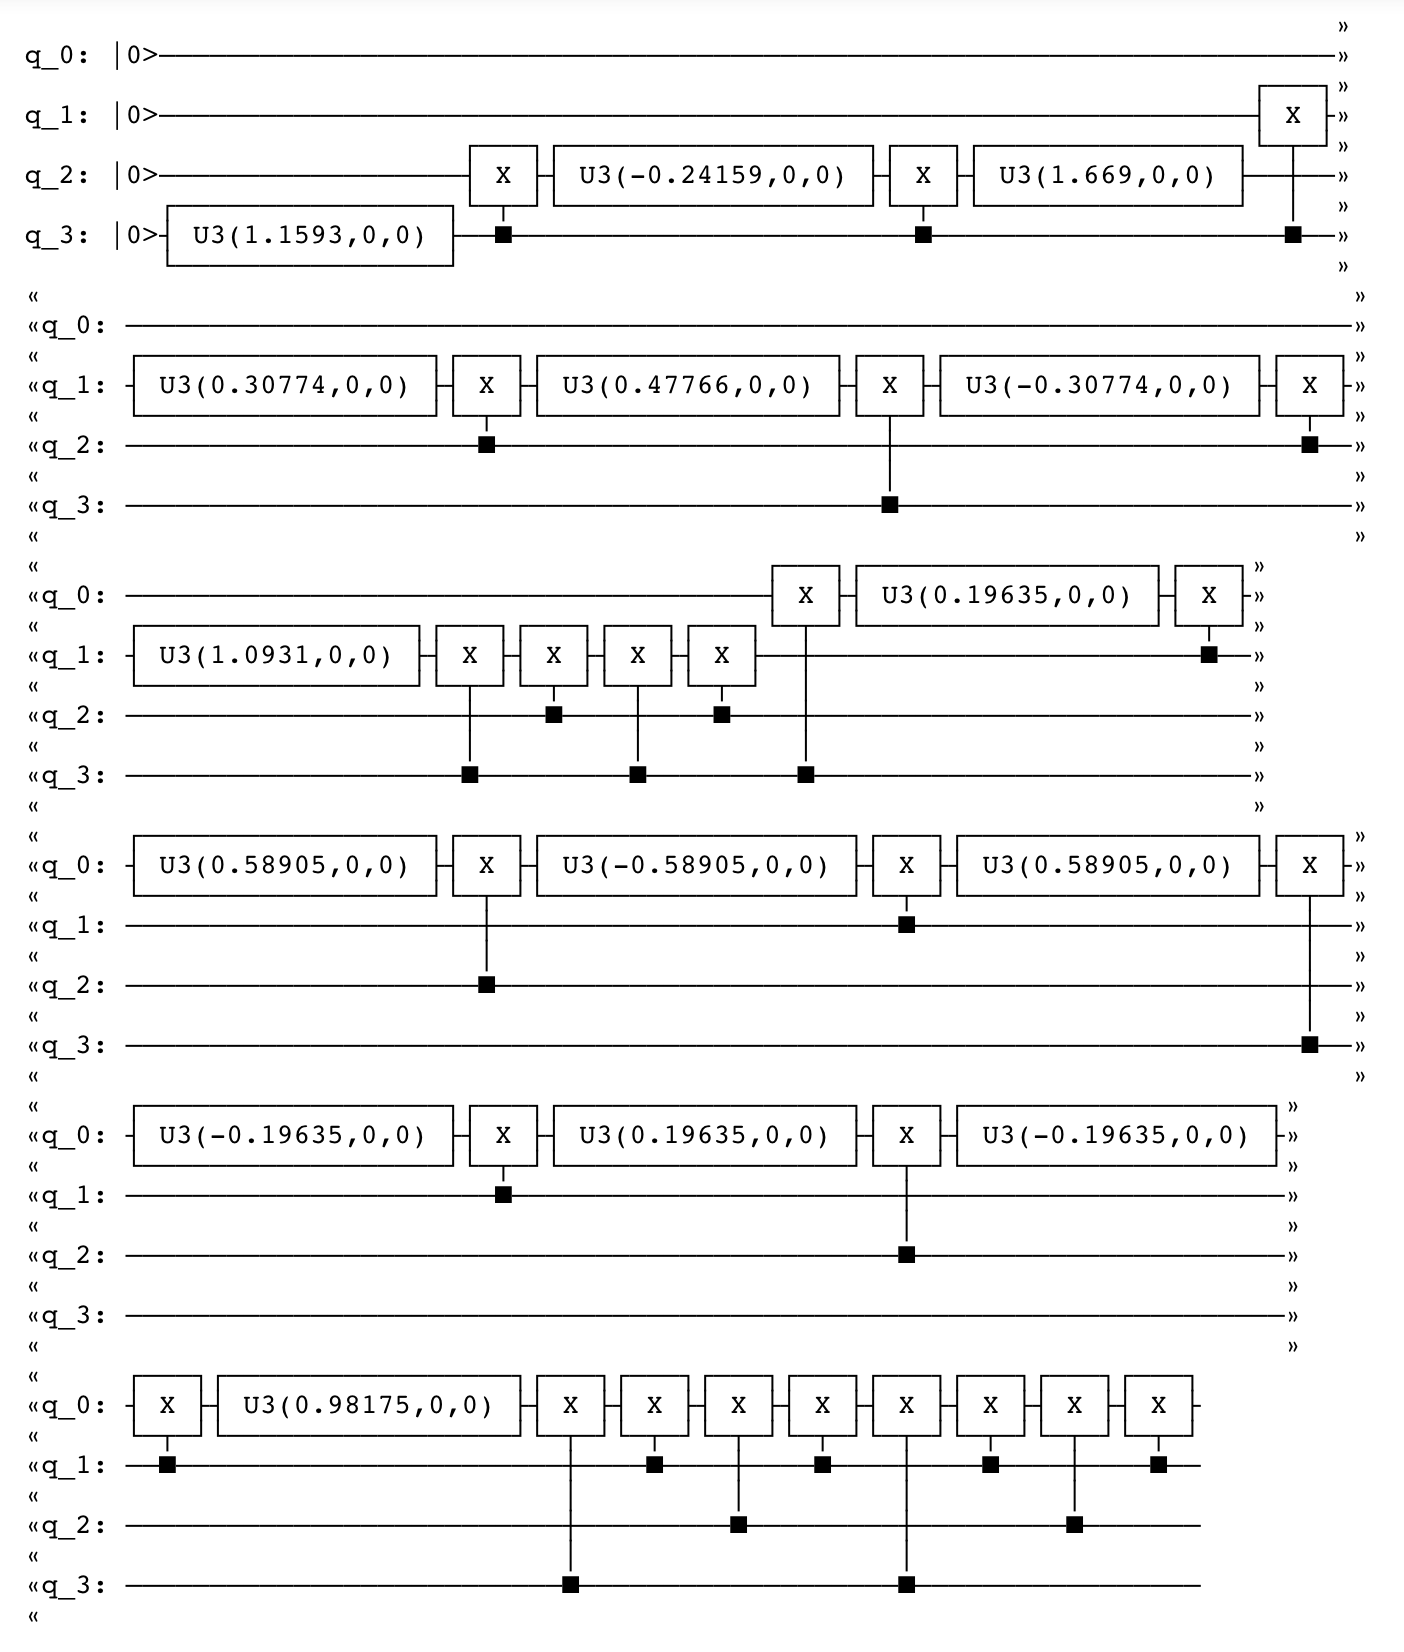
\includegraphics{../img/circ.png}
\caption{The circuit for a 4x4 image.}
\end{figure}

    \hypertarget{the-hadamard-gate-with-more-than-2-pixels}{%
\section{The Hadamard gate with more than 2
pixels}\label{the-hadamard-gate-with-more-than-2-pixels}}

    Recall that the Hadamard gate has the following effect on the zero and
one basis states:

\(H|0\rangle \rightarrow (|0\rangle + |1\rangle)/\sqrt{2}\)

\(H|1\rangle \rightarrow (|0\rangle - |1\rangle)/\sqrt{2}\)

Consider a four pixel image, represented with two qubits, and what
happens when a Hadamard gate is applied to just the last qubit. We'll
subscript the Hadamard operator to tell which qubit it's acting on.

\[ |\textrm{image}\rangle = \alpha_{00}|00\rangle + \alpha_{01}|01\rangle + \alpha_{10}|10\rangle + \alpha_{11}|11\rangle \]

\[ |\textrm{image}\rangle = \alpha_{00}|0\rangle|0\rangle + \alpha_{01}|0\rangle|1\rangle + \alpha_{10}|1\rangle|0\rangle + \alpha_{11}|1\rangle|1\rangle \]

\[ \sqrt{2} H_0 |\textrm{image}\rangle = \alpha_{00}|0\rangle \sqrt{2} H |0\rangle + \alpha_{01}|0\rangle \sqrt{2} H|1\rangle + \alpha_{10}|1\rangle \sqrt{2} H|0\rangle + \alpha_{11}|1\rangle\sqrt{2} H|1\rangle\]

\[ \sqrt{2} H_0 |\textrm{image}\rangle = \alpha_{00}|0\rangle(|0\rangle + |1\rangle) + \alpha_{01}|0\rangle(|0\rangle - |1\rangle) + \alpha_{10}|1\rangle(|0\rangle + |1\rangle) + \alpha_{11}|1\rangle(|0\rangle - |1\rangle)\]

\[ \sqrt{2} H_0 |\textrm{image}\rangle = \alpha_{00}(|00\rangle+|01\rangle) + \alpha_{01}(|00\rangle-|01\rangle) + \alpha_{10}(|10\rangle+|11\rangle) + \alpha_{11}(|10\rangle-|11\rangle) \]

\[ \sqrt{2} H_0 |\textrm{image}\rangle = (\alpha_{00} + \alpha_{01})|00\rangle + (\alpha_{00} - \alpha_{01})|01\rangle + (\alpha_{10} + \alpha_{11})|10\rangle + (\alpha_{10} - \alpha_{11})|11\rangle \]

    \[ \sqrt{2} H_0 |\textrm{image}\rangle = (\alpha_{00} + \alpha_{01})|00\rangle + (\alpha_{00} - \alpha_{01})|01\rangle + (\alpha_{10} + \alpha_{11})|10\rangle + (\alpha_{10} - \alpha_{11})|11\rangle \]

What happens to the state above if we measure just the state of the
first qubit and happen to get the result \(1\)? The state of the second
qubit will still be undetermined, but the system's overall state vector
would be made up of only those states consistent with our first
measurement: \(|01\rangle\) and \(|11\rangle\). So, if the first
measurement results in a 1, it must shrink, or \emph{collapse}, the
state down to one proportional to

\[ |\textrm{final state}\rangle = (\alpha_{00} - \alpha_{01})|01\rangle + (\alpha_{10} - \alpha_{11})|11\rangle \]

which holds just the edge information we're interested in.

    \hypertarget{implementing-the-algorithm}{%
\section{Implementing the
algorithm}\label{implementing-the-algorithm}}

Beginning with the circuit \texttt{circ} that generates the image's
state vector representation, apply the Hadamard gate to \emph{just} the
first qubit.

    \begin{Verbatim}[commandchars=\\\{\}]
{\color{incolor}In [{\color{incolor}7}]:} \PY{n}{circ}\PY{o}{.}\PY{n}{h}\PY{p}{(}\PY{n}{qr}\PY{p}{[}\PY{l+m+mi}{0}\PY{p}{]}\PY{p}{[}\PY{l+m+mi}{0}\PY{p}{]}\PY{p}{)}
\end{Verbatim}


\begin{Verbatim}[commandchars=\\\{\}]
{\color{outcolor}Out[{\color{outcolor}7}]:} <qiskit.extensions.standard.h.HGate at 0x1c25585358>
\end{Verbatim}
            
    Simulate the circuit using the \texttt{StatevectorSimulator} and read
the resulting state vector.

    \begin{Verbatim}[commandchars=\\\{\}]
{\color{incolor}In [{\color{incolor}8}]:} \PY{k+kn}{from} \PY{n+nn}{qiskit} \PY{k}{import} \PY{n}{BasicAer}\PY{p}{,} \PY{n}{execute}
\end{Verbatim}


    \begin{Verbatim}[commandchars=\\\{\}]
{\color{incolor}In [{\color{incolor}9}]:} \PY{n}{simulator}   \PY{o}{=} \PY{n}{BasicAer}\PY{o}{.}\PY{n}{get\PYZus{}backend}\PY{p}{(}\PY{l+s+s1}{\PYZsq{}}\PY{l+s+s1}{statevector\PYZus{}simulator}\PY{l+s+s1}{\PYZsq{}}\PY{p}{)}
        \PY{n}{sim\PYZus{}result}  \PY{o}{=} \PY{n}{execute}\PY{p}{(}\PY{n}{circ}\PY{p}{,} \PY{n}{simulator}\PY{p}{)}\PY{o}{.}\PY{n}{result}\PY{p}{(}\PY{p}{)}
        \PY{n}{final\PYZus{}state} \PY{o}{=} \PY{n}{sim\PYZus{}result}\PY{o}{.}\PY{n}{get\PYZus{}statevector}\PY{p}{(}\PY{n}{circ}\PY{p}{)}
\end{Verbatim}


    \hypertarget{decode-the-state-vector-back-into-an-image}{%
\section{Decode the state vector back into an
image}\label{decode-the-state-vector-back-into-an-image}}

    To turn the state vector back into an image, read off the \(\alpha\)'s
and reshape the column vector back into a matrix.

    \begin{Verbatim}[commandchars=\\\{\}]
{\color{incolor}In [{\color{incolor}10}]:} \PY{n}{edge}   \PY{o}{=} \PY{n}{np}\PY{o}{.}\PY{n}{real}\PY{p}{(}\PY{n}{final\PYZus{}state}\PY{p}{)}
         \PY{n}{n\PYZus{}rows} \PY{o}{=} \PY{n+nb}{int}\PY{p}{(}\PY{n}{np}\PY{o}{.}\PY{n}{sqrt}\PY{p}{(}\PY{n+nb}{len}\PY{p}{(}\PY{n}{edge}\PY{p}{)}\PY{p}{)}\PY{p}{)}
         \PY{n}{n\PYZus{}cols} \PY{o}{=} \PY{n}{n\PYZus{}rows}
         \PY{n}{edge}   \PY{o}{=} \PY{n}{edge}\PY{o}{.}\PY{n}{reshape}\PY{p}{(}\PY{n}{n\PYZus{}rows}\PY{p}{,} \PY{n}{n\PYZus{}cols}\PY{p}{)}
\end{Verbatim}


    The edges are indicated by the basis states where the first qubit is
\(1\). After decoding the 1-D state vector back into a 2-D image, these
basis states are the 2-D image's even columns. To retain only these
columns, zero out the odd columns.

    \begin{Verbatim}[commandchars=\\\{\}]
{\color{incolor}In [{\color{incolor}11}]:} \PY{n}{edge}\PY{p}{[}\PY{p}{:}\PY{p}{,}\PY{p}{:}\PY{p}{:}\PY{l+m+mi}{2}\PY{p}{]} \PY{o}{=} \PY{l+m+mi}{0}
\end{Verbatim}


    Display the edges and the original image for comparison.

    \begin{Verbatim}[commandchars=\\\{\}]
{\color{incolor}In [{\color{incolor}12}]:} \PY{n}{fig}\PY{p}{,} \PY{n}{ax} \PY{o}{=} \PY{n}{plt}\PY{o}{.}\PY{n}{subplots}\PY{p}{(}\PY{l+m+mi}{1}\PY{p}{,}\PY{l+m+mi}{2}\PY{p}{)}
         \PY{n}{ax}\PY{p}{[}\PY{l+m+mi}{0}\PY{p}{]}\PY{o}{.}\PY{n}{imshow}\PY{p}{(}\PY{n}{edge}\PY{p}{)}
         \PY{n}{ax}\PY{p}{[}\PY{l+m+mi}{1}\PY{p}{]}\PY{o}{.}\PY{n}{imshow}\PY{p}{(}\PY{n}{im}\PY{p}{)}
\end{Verbatim}


\begin{Verbatim}[commandchars=\\\{\}]
{\color{outcolor}Out[{\color{outcolor}12}]:} <matplotlib.image.AxesImage at 0x1c25c84e80>
\end{Verbatim}
            
    \begin{center}
    \adjustimage{max size={0.9\linewidth}{0.9\paperheight}}{../img/output_34_1.png}
    \end{center}
    { \hspace*{\fill} \\}
    
    Notice we've only found the edges in every other column of the image. A
modification of the QHED algorithm can find the edges in all columns
with a single circuit, as described in
\href{https://journals.aps.org/prx/abstract/10.1103/PhysRevX.7.031041}{Yao,
Xi-Wei et al., Quantum Image Processing and Its Application to Edge
Detection: Theory and Experiment, Phys. Rev.~X 7, 031041, (2017)}.


    % Add a bibliography block to the postdoc
    
    
    
    \end{document}
